% --- [ Type Lattice ] ---------------------------------------------------------

\subsection{Type Lattice}

A type lattice may be thought of as a set of subtyping relationships, represented as a directed graph from the \textit{top} type $\top$ to the \textit{bottom} type $\bot$; where every type is a subtype of $\top$, and no type is a subtype of $\bot$.

\begin{itemize}
	\item $\top$: any type
	\item $\bot$: inconsistent type
\end{itemize}

In the primitive type lattice of TIE (see figure \ref{fig:primitive_type_lattice}) for instance, both signed and unsigned 32-bit integers (\texttt{int32} and \texttt{uint32}, respectively) are subtypes of 32-bit integers (\texttt{num32}) \cite{tie_reverse_engineering_of_types}.

\begin{figure}[htbp]
	\centering
	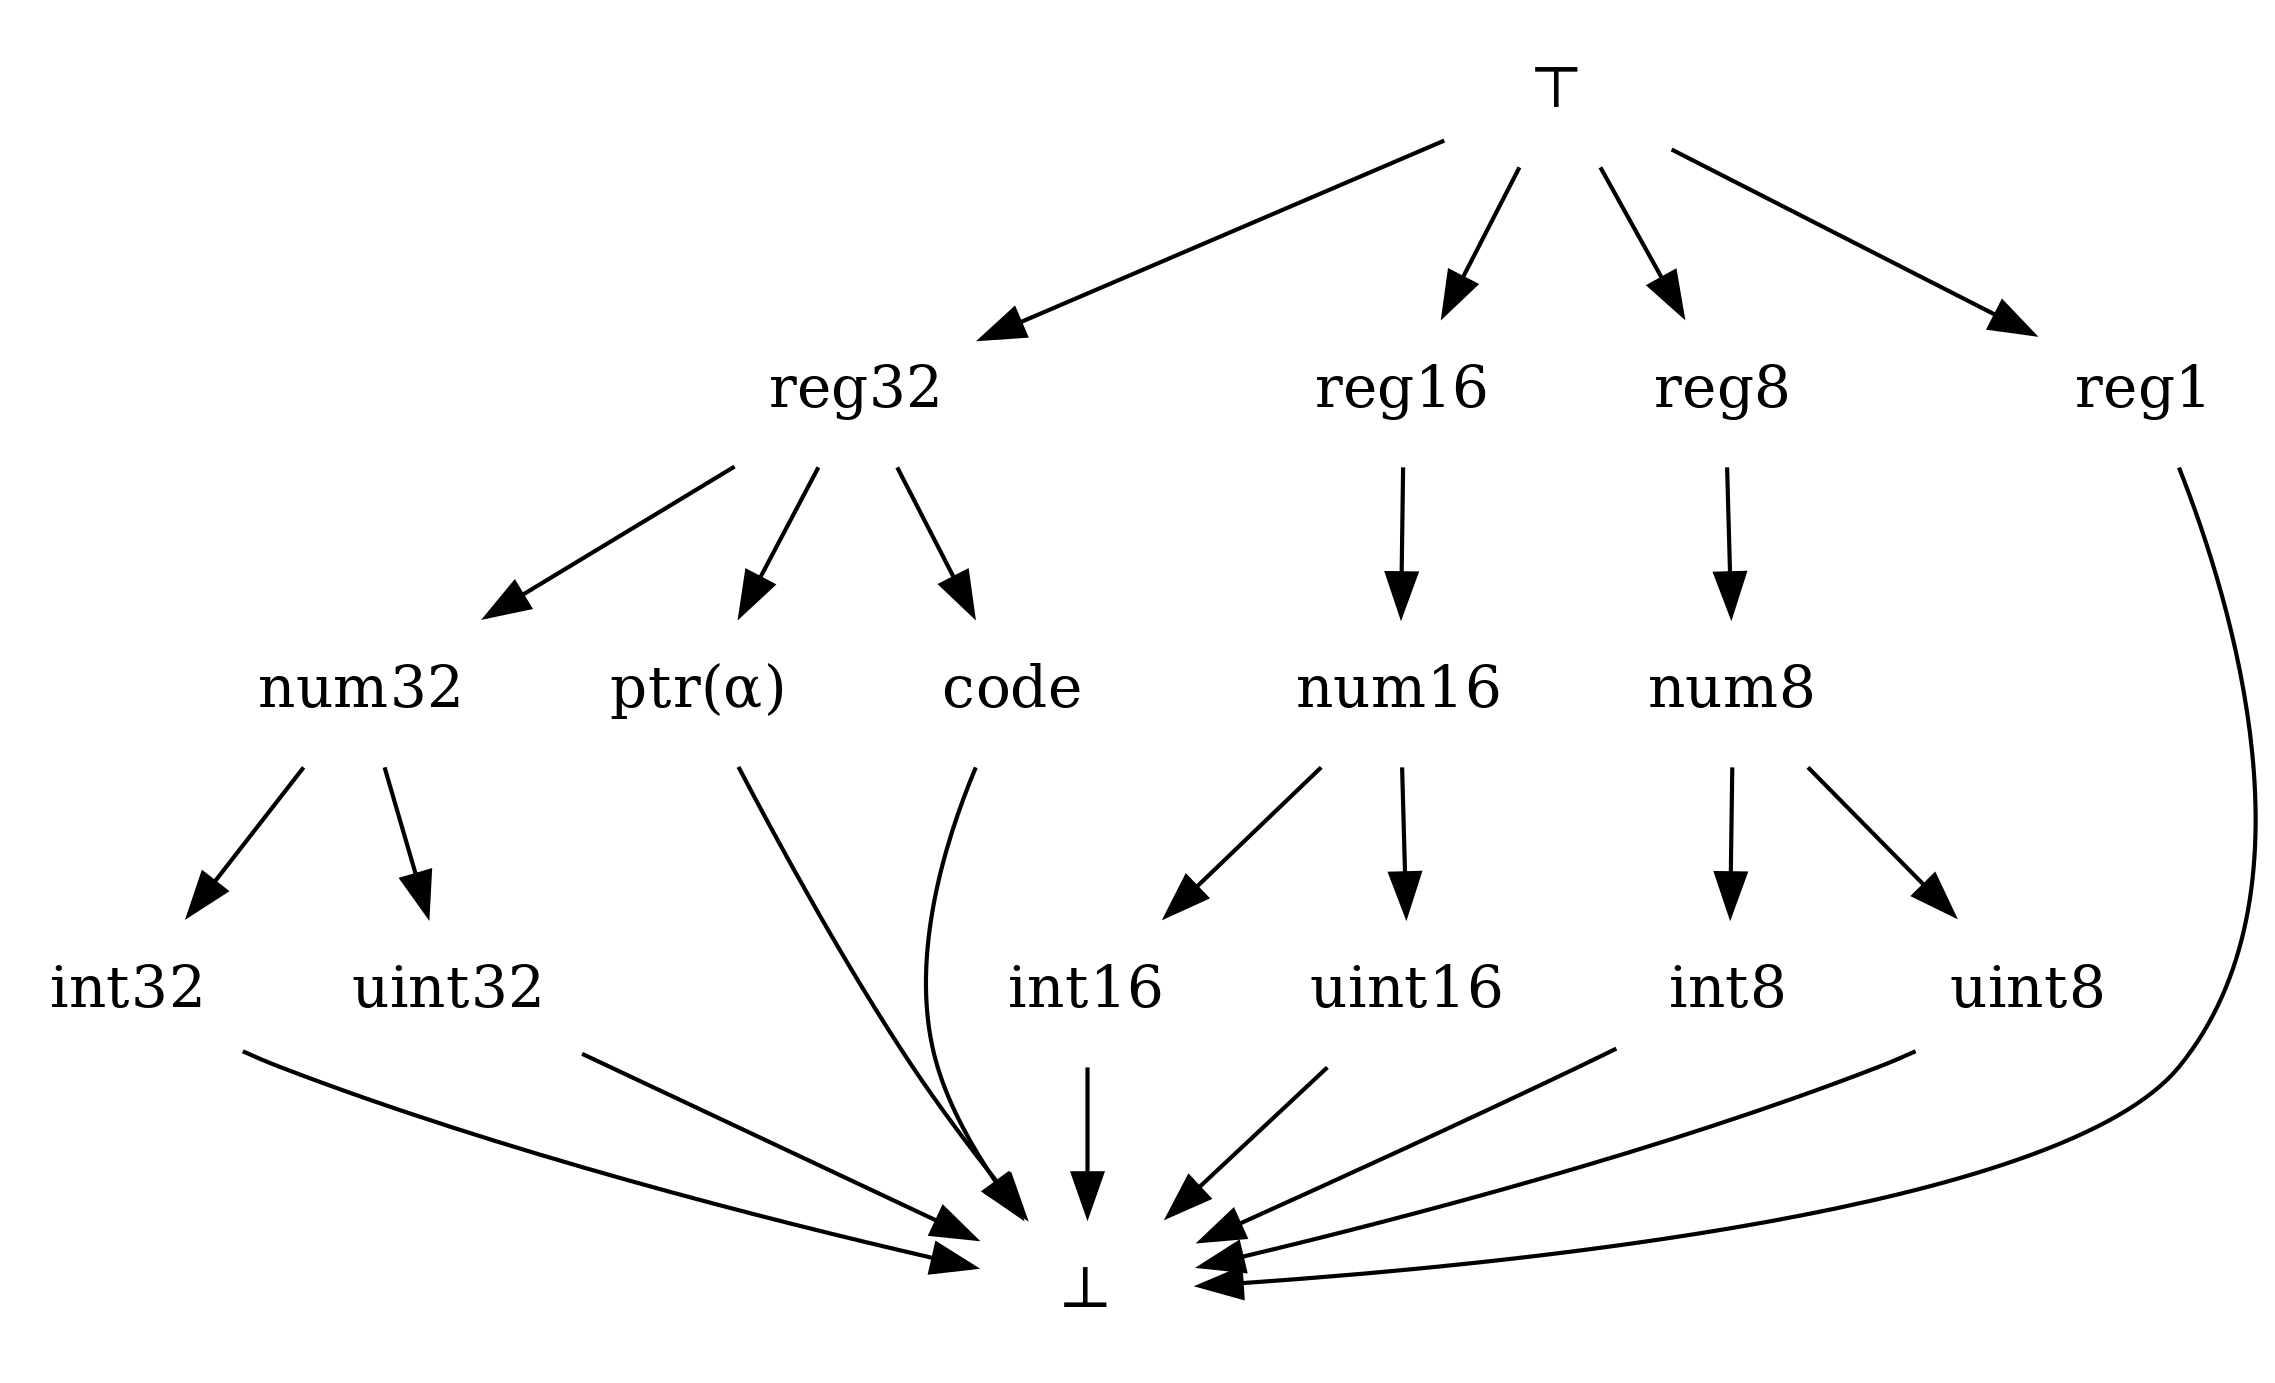
\includegraphics[width=0.40\textwidth]{inc/tie_primitive_type_lattice.png}
	\caption{Primitive type lattice of TIE.}
	\label{fig:primitive_type_lattice}
\end{figure}

In the context of type recovery, a type lattice may be used to specify the set of possible types for a variable through upper and lower bounds; thus imposing type constraints on the variable.
